\documentclass[12pt,a4paper]{article}

%%%%%%%%%%%%%%%%%%%%%%%%% packages %%%%%%%%%%%%%%%%%%%%%%%%
\usepackage{amsmath}
\usepackage{amssymb}
\usepackage{amsthm}
\usepackage{amsfonts}
\usepackage{graphicx}
\usepackage[utf8]{inputenc}
\usepackage[english]{babel}
\usepackage[all]{xy}
\usepackage{float}
\usepackage{tikz}
\usepackage{verbatim}
\usepackage[left=2cm,right=2cm,top=2cm,bottom=2cm]{geometry}
\usepackage{hyperref}
\usepackage{caption}
\usepackage{subcaption}
\usepackage{psfrag}


%%%%%%%%%%%%%%%%%%%%% students data %%%%%%%%%%%%%%%%%%%%%%%%
\newcommand{\student}{Brian KYANJO }
\newcommand{\course}{Parallel Scientific Computing}
\newcommand{\assignment}{Final}

%%%%%%%%%%%%%%%%%%% using theorem style %%%%%%%%%%%%%%%%%%%%
\newtheorem{thm}{Theorem}
\newtheorem{lem}[thm]{Lemma}
\newtheorem{defn}[thm]{Definition}
\newtheorem{definition}{Definition}[section] 
\newtheorem{theorem}{Theorem}
\newtheorem{exa}[thm]{Example}
\newtheorem{rem}[thm]{Remark}
\newtheorem{coro}[thm]{Corollary}
\newtheorem{quest}{Question}[section]

%%%%%%%%%%%%%%  Shortcut for usual set of numbers  %%%%%%%%%%%

\newcommand{\N}{\mathbb{N}}
\newcommand{\Z}{\mathbb{Z}}
\newcommand{\Q}{\mathbb{Q}}
\newcommand{\R}{\mathbb{R}}
\newcommand{\C}{\mathbb{C}}

%%%%%%%%%%%%%%%%%%%%%%%%%%%%%%%%%%%%%%%%%%%%%%%%%%%%%%%
\begin{document}
	
	%%%%%%%%%%%%%%%%%%%%%%% title page %%%%%%%%%%%%%%%%%%%%%%%%%%
	\thispagestyle{empty}
	\begin{center}
		\textbf{BOISE STATE UNIVERSITY \\[0.5cm]
			(BSU, USA)}
		\vspace{.2cm}
	\end{center}
	
	%%%%%%%%%%%%%%%%%%%%% assignment information %%%%%%%%%%%%%%%%
	\noindent
	\rule{17cm}{0.2cm}\\[0.3cm]
	Name: \student \hfill Project Number: \assignment\\[0.1cm]
	Course: \course \hfill Date: \today\\
	\rule{17cm}{0.05cm}
	\vspace{.2cm}

\section*{Problem description}
Monte Carlo integration to estimate the integral:
$$\int_{0}^{\infty} e^{-\lambda x} \cos x dx $$

 \noindent for $\lambda > 0$ by using an exponential distribution $p(x) = \lambda e^{- \lambda x}$ for $x \ge 0,$ which has a variance $var\{p(x)\} = \frac{1}{\lambda^{2}}$ . Where X is a random value obtained from a uniform distribution on the interval $[0,1]$, with random variable Y drawn from $p(x)$ can be obtained by transformation:
 $$Y = -\frac{1}{\lambda} \ln X$$
 
 The exact value of the integral is given by;
 $$\int_{0}^{\infty} e^{-\lambda x} \cos x dx = \frac{\lambda}{1 + \lambda^{2}} $$

\section*{Task 1 - Monte Carlo integration with MPI}
The  problem  has been programed using MPI. And the code takes $N$ samples as an input parameter. The entire program has been measured  using MPI\textunderscore Wtime function.

\begin{enumerate}
	\item I used $\lambda = 1$, and the number of samples ($N = 10^{10}$), required to achieve  an error tolerance $\epsilon = 10^{-5} $ with 99\% confidence in the code named \textbf{mc\textunderscore task1\textunderscore 2.c}. This code was run with the determined  N, and the solution was achieved as shown in figure \ref{fig:t11} below. 
	
	\begin{figure}[H]
		\centering
		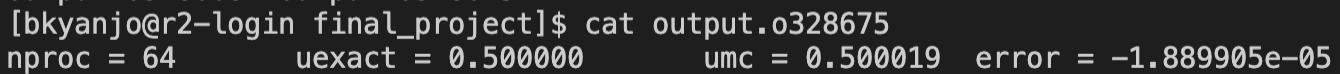
\includegraphics[width=0.7\linewidth]{t11}
		\caption{Verification of the solution against the exact solution.}
		\label{fig:t11}
	\end{figure}
	Note: I performed many simulations on the problem with different the number of processors, but the best confidence error from the exact solution, depended on the Number of samples rather than the number of processors. This led me to use just $64$ processors, since its even considered as the upper bound in next parts of the question.
	
	
\item The computational time required to obtain a solution for $N = 10^{q}$ samples, where $q = 3,4,5,6,7,8,9,10$ was measured in the code named \textbf{mc\textunderscore task1\textunderscore 1.c}, and results for Time against N was measured and plotted as shown in figure \ref{fig:t12}. 

	\begin{figure}[H]
	\centering
	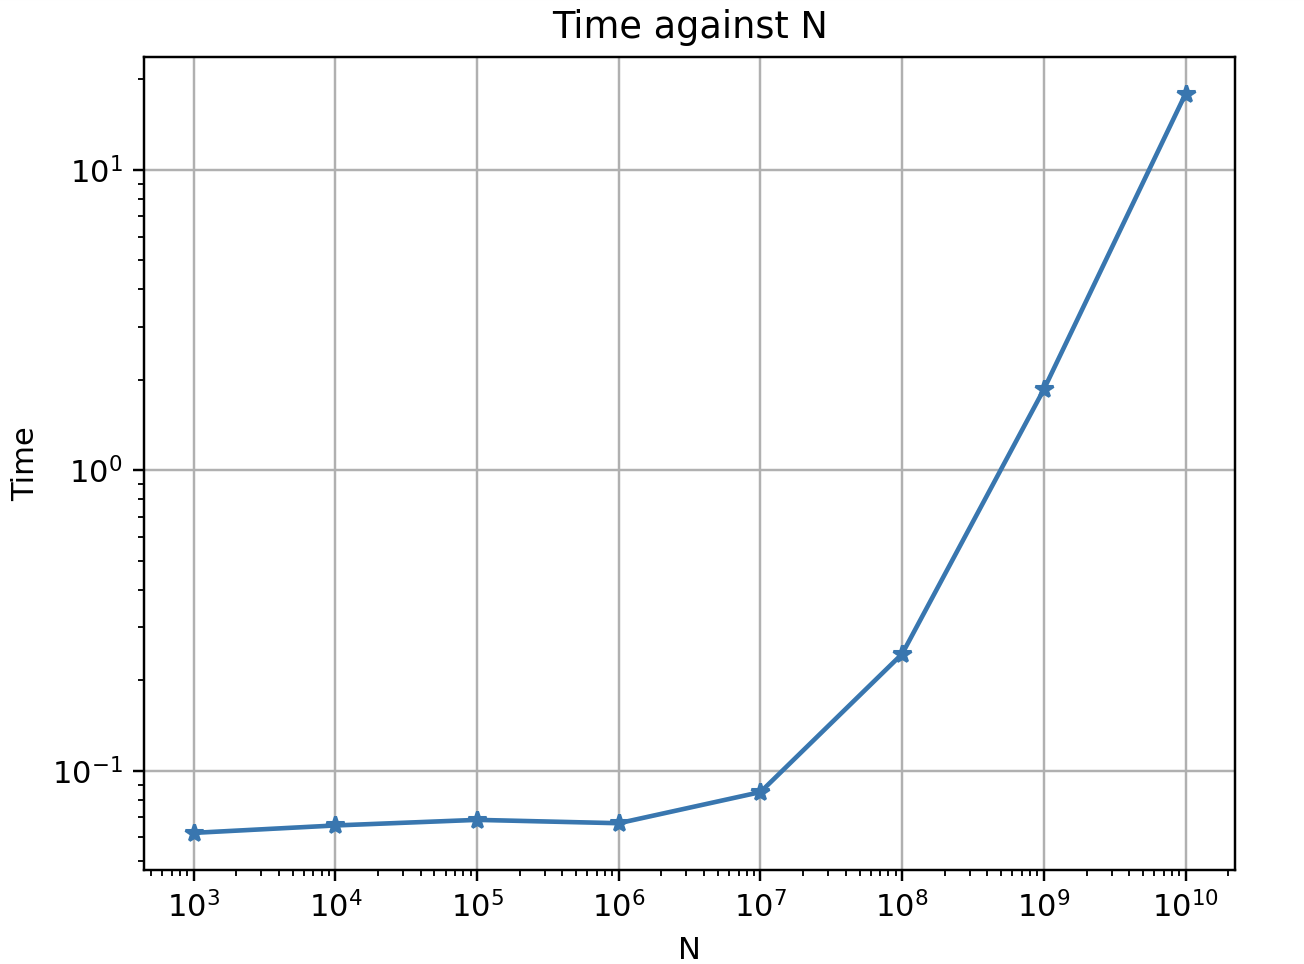
\includegraphics[width=0.7\linewidth]{t12}
	\caption{Time evaluation plot for the MPI code}
	\label{fig:t12}
\end{figure}

Figure \ref{fig:t12}, depicts that computational time is small for number of samples between $10^{3}$ and $10^{7}$, but after that increases with increase in N. This is because large number of samples require more resouces than smaller one, so much time is spent on the loops that generate random samples for these bigger problem size. Making computational time expensive.  However, large samples have proved to produce the most effective results in accordance to smaller ones.

According to figure \ref*{fig:error}, the red dotted horizontal line straches up to the y-axis, which gives us the estimate of the time reqired to obtain a tolerance of  $10^{-5}$ with  $N=10^{10}$, this estimated  time is $15.667943$ seconds. 

	\begin{figure}[H]
	\centering
	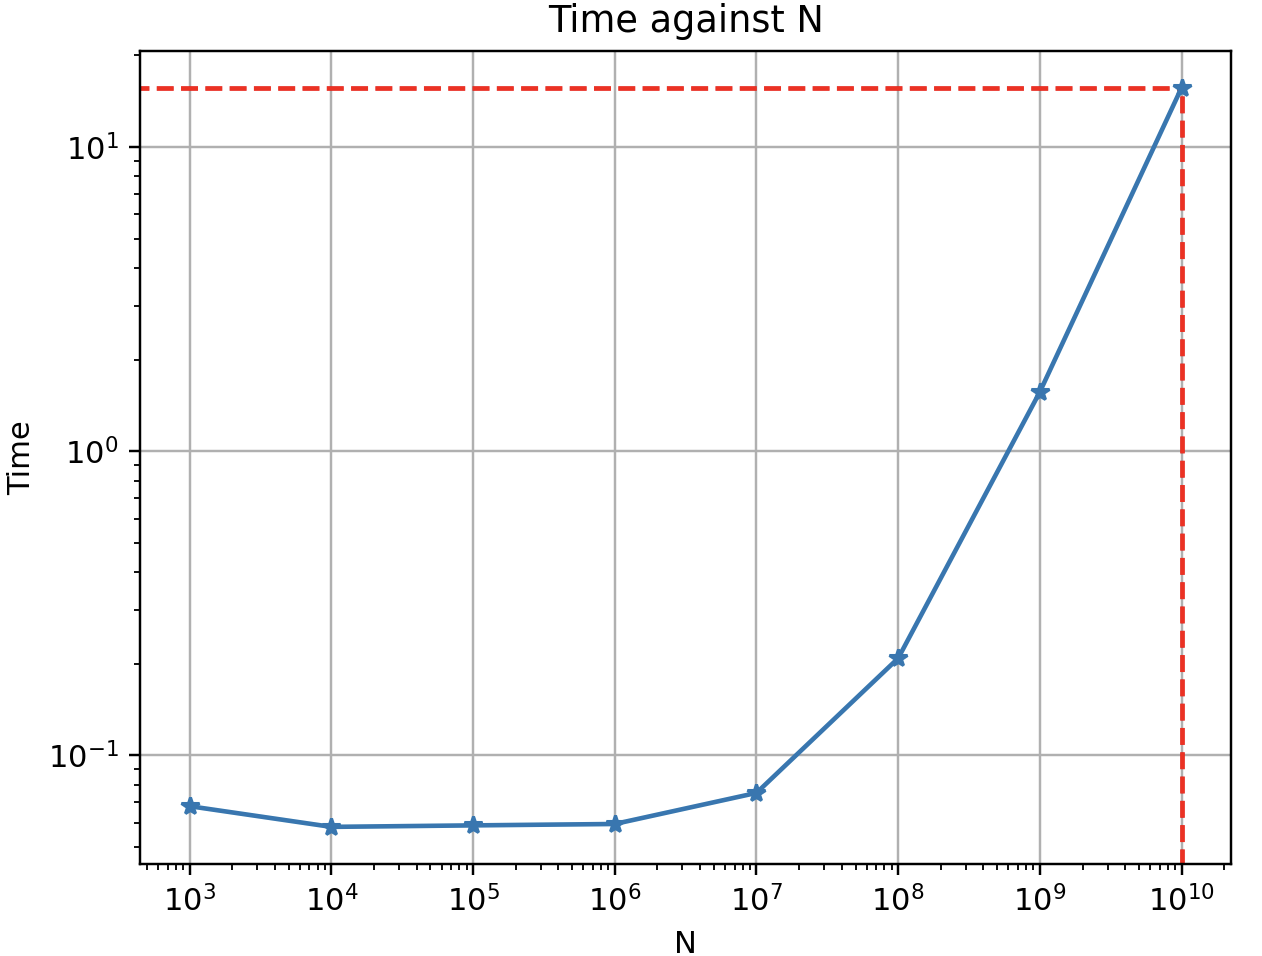
\includegraphics[width=0.7\linewidth]{error}
	\caption{Estimated time to reach a tolerance of  $10^{-5}$  }
	\label{fig:error}
\end{figure}


\item Strong scaling plots for $p = 1, 2, 4, 8, 16, 32, 64$ processors have been created using a problem size $N=2^{28}$ which is upper bound for the $p = 64$ processors in the weak scaling simulations. The speedup and efficiency plots for the strong sclaing simulation have been plotted and displayed in figures \ref{fig:speedup_task1} and \ref{fig:t1e} respectively.

Figure \ref{fig:speedup_task1} depict linear scaling for number of processors:$ 1, 2, 4, $ and $8$ after which scaling drops. This means that the program was perfectly scaled up to $8$  processors then attains typical sucess for the remaining processors. Which implies that the upper limit for the scaled speedup is attained at $8$ processes, and that's when each process is contributing 100\% of its computational power.

Figure \ref{fig:t1e} shows that as the number of processors increase with fixed problem size, parallel efficiency exceeds 100\%, for the first resourse, this is due to minimized load imbalance and overhead, and maximized concurency. After that as the number of processors increase with a fixed problem size,  parallel efficiency drops gradually. This is because according to Amdahl's law as the number of processors increases, with a fixed problem size, and running the program on a single processor(serial time), since some part of the code where not parallelized, the time taken by the parallelized fraction of the code, for what ever number of processors used, cannot be less than the execution time by the serial part, hence as the processes increases, parallel efficiency decreases, however, it sustains the efficiency good enough  that it  only droped to below $80\%.$  

\begin{figure}[h]
	\begin{subfigure}[b]{0.5\textwidth}
		\centering
		\includegraphics[width=1.0\linewidth]{"t1s"}
		\caption{}
		\label{fig:speedup_task1}
	\end{subfigure}
	%
	\begin{subfigure}[b]{0.5\textwidth}
		\centering
		\includegraphics[width=1.0\linewidth]{"t1e"}
		\caption{}
		\label{fig:t1e}
	\end{subfigure}
	\caption{(a) and (b) respectively show speedup and Efficiency plots for strong scaling Task1. }
\end{figure}

A weak scaling plot for $p = 1, 2, 4, 8, 16, 32, 64$ processors has been created with doubling the problem size starting at $N=2^{22}$  to $N=2^{28}$ which is the  problem size used in performing strong scaling simulations. This means that both figures \ref{fig:t1e} and \ref{fig:t1we} have the same end point on the plot. The efficiency plot for the weak scaling  simulation has been ploted as shown in figure \ref{fig:t1we}.

Figure \ref{fig:t1we} depicts that the code was $100\%$ parallel efficiencient for the first three simulations as the problem size doubles, after which  it  drops gradually with increasing number of processors, as the problem size doubles. This implies that this program has been made cost optimal, hence the system sustained efficiency, good enough  almost all the runs it was better than strong scaling. This is much possible due to the right allocation of available resources efficitiently to the right problem size hence good efficiency satisfying Gustafson's law.

\begin{figure}[H]
	\centering
	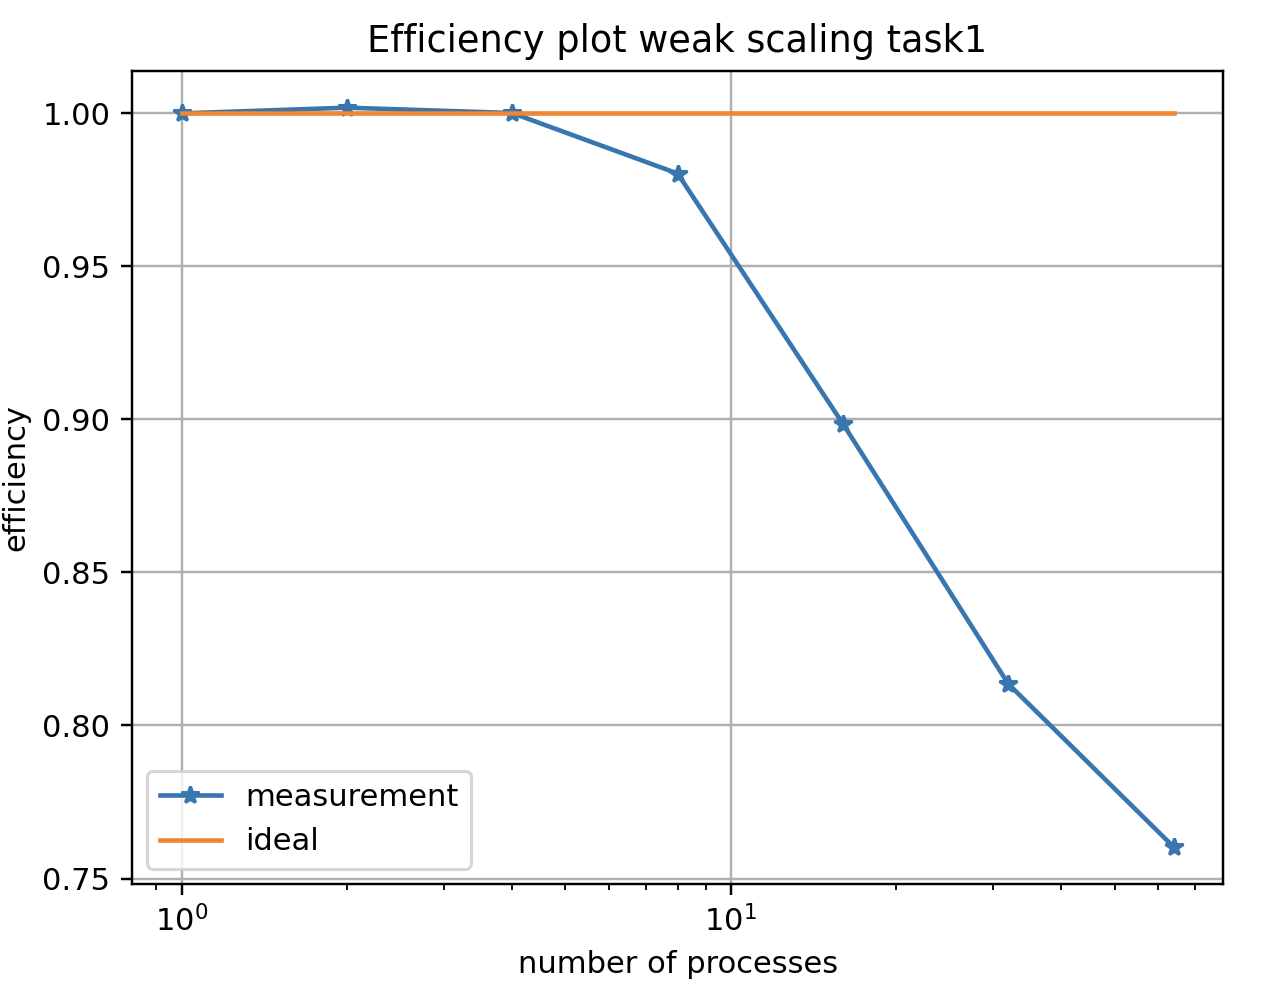
\includegraphics[width=0.7\linewidth]{t1we}
	\caption{Weak scaling parallel efficiency}
	\label{fig:t1we}
\end{figure}
\end{enumerate}

\section*{Task 2 - Monte Carlo integration with CUDA}
The MPI-Monte Carlo integration problem in the previous has been implemented using CUDA. In a similar way like in Task1, the program named \textbf{mc\textunderscore task2.cu} has been implemented and was tested using $\lambda = 1$  with  $N= 10^{10}$, which gave a tolerance of $10^{-5}$ with confidence $99\%$, as shown in figure \ref{fig:t2} below.

\begin{figure}[H]
	\centering
	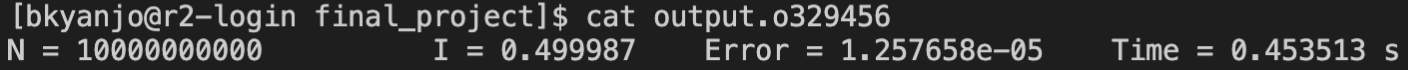
\includegraphics[width=0.7\linewidth]{t2}
	\caption{Results obtained using $\lambda = 1$  with  $N= 10^{10}$ }
	\label{fig:t2}
\end{figure}

\noindent The time required to compute a solution for $N=10^{q}$ samples has been measured and ploted versus $N$. The results has been compared to MPI results as shown in figure \ref{fig:cudampi}.  For $N \le 10^{8} $, MPI performs better than Cuda. However this is because 
of the cost of setup time in the cuda code  according to figure \ref{fig:t2n} for $N \le 10^{8}$ than the MPI code. According to Cuda tool kit  (\cite{cuda}), its written that cudaMalloc is expensive, hence may affect performance comparisions, so therefore excluding setup time makes comparision reasonable and exposes cudas power over MPI (figure \ref{fig:t2n}). Hence, Cuda performs much better than MPI, and in that very figure, generally its also observed that computational time evolution with increasing problem size trend is well exhibited.\\

\noindent Due to the fact that the choice of threads per block influences occupancy and matching the problem size, the restriction of $65535$ blocks per grid dimesion which are not large enough to create enough threads to cover large N values. So observing that threads per block should be a multiple of $32$,  since the kernel gives instructions in wraps ($32$ threads) \cite{10.5555/2430671}. I decided to use $128$ threads per block so that i can be able to fit necessary blocks in my streaming multiprocessors before hitting the maximum  $65535$ blocks. In this way atleast maximizing occupancy, eventhough not enough threads may be created to cover lage N values.

\begin{figure}[H]
	\begin{subfigure}[b]{0.5\textwidth}
		\centering
		\includegraphics[width=1.0\linewidth]{"cuda_mpi"}
		\caption{}
		\label{fig:cudampi}
	\end{subfigure}
	%
	\begin{subfigure}[b]{0.5\textwidth}
		\centering
		\includegraphics[width=1.0\linewidth]{"t2n"}
		\caption{}
		\label{fig:t2n}
	\end{subfigure}
	\caption{(a) and (b) respectively show the comparision of Cuda results against MPI  with and without allocation of memory taken into account.}
\end{figure}

\noindent The number of blocks per each problem size $N$, was computed using the equation \eqref{1};

\begin{equation}
	B = \dfrac{N + T -1 }{T}
	\label{1}
\end{equation}
where B is the number of blocks, N is the problem size, T is the threads per block. However $B$ is restricted not exceed $65535$ blocks, so for any $N$ that makes $B \ge 65535$, a default value of $B= 65535$ is used in the simulation.

\section*{Task 3 - Reduction operation in CUDA}

The reduction kernel was implemented in the Cuda code named \textbf{mc\textunderscore task3.cu}, and the computation time was measured and ploted against previous results as shown in figure \ref{fig:combined} with memory allocation taken into account. \\

\noindent Figures \ref{fig:combined} and \ref{fig:t3nm_3} represent time evolution with increasing problem size $N$, for MPI, task2 and 3 Cuda results with and without allocation of memory respectively. In figure \ref{fig:combined}, the time evolution for $N\le10^{8}$ depicts a very infinitesimal change for the two simulations: task2 and 3, making MPI to win with cheap execution time. This kind of behaviour is due to the fact that setup time is expensive, and since for $N\le10^{8}$, the computational time is very small, then the setup time dominats and we can't really see the difference, however when these two graphs are plotted independently, without MPI, we see a potential time change. For values $N>10^{8}$, Cuda simulations performs better than MPI. \\

\noindent After implementation of the reduction kernel to replace atomicAdd, we see an overal  improvemnet in the computational time, and the tolence too was improved for task3 compared to task2. This is because the butterfly sumation implemented uses parallel reduction which is,  way faster and converges to a better solution than the serial atomicAdd.\\

\noindent However, observing figure \ref{fig:t3nm_3}, where setup time is not taken into account, the performance for the three simulations is well exhibitted, and the time evolution for all of them is well exposed as $N$ shoots up. In this case the strength of the implemented reduction kernel to replace the atomicAdd, is well felt, as we can see that task3 simulation (green) wins out for the entire simulations. I therefore conclude that implemtation of the reduction kernel improved the device performace. 



\begin{figure}[H]
	\begin{subfigure}[b]{0.5\textwidth}
		\centering
		\includegraphics[width=1.0\linewidth]{"combined"}
		\caption{}
		\label{fig:combined}
	\end{subfigure}
	%
	\begin{subfigure}[b]{0.5\textwidth}
		\centering
		\includegraphics[width=1.0\linewidth]{"t3nm_3"}
		\caption{}
		\label{fig:t3nm_3}
	\end{subfigure}
	\caption{(a) and (b) respectively show the comparision of Cuda results (task2 and 3),  against MPI  with and without allocation of memory taken into account.}
\end{figure}


	\bibliographystyle{plain}
	\bibliography{document}
	
\end{document}